% Capítulo 2: etapas da compilação de um programa C++.
\documentclass[border=4pt]{standalone}
\usepackage[utf8]{inputenc}
\usepackage[T1]{fontenc}
% Estilo comum dos fluxogramas e diagramas de blocos.
\usepackage{tikz}
\usetikzlibrary{arrows.meta, positioning, calc, shapes.geometric, shapes.misc}
\definecolor{navy}{RGB}{23,45,80}
\definecolor{laranja}{RGB}{250,110,29}
\definecolor{cinzalogo}{RGB}{107,114,126}
\definecolor{azul}{RGB}{205,222,247}
\tikzset{
  base/.style={draw=navy, line width=0.9pt, font=\sffamily\small, align=center, inner sep=4pt},
  terminal/.style={base, rounded rectangle, fill=laranja!45, draw=laranja, minimum width=20mm, minimum height=7mm},
  processo/.style={base, rectangle, fill=laranja!12, minimum width=28mm, minimum height=8mm},
  decisao/.style={base, diamond, aspect=2.2, fill=azul, inner sep=1pt, minimum width=30mm},
  es/.style={base, trapezium, trapezium left angle=72, trapezium right angle=108,
             fill=white, minimum width=26mm, minimum height=8mm, trapezium stretches body},
  fluxo/.style={-{Stealth[length=2.2mm]}, navy, line width=0.9pt},
  rotulo/.style={font=\sffamily\small\bfseries, text=navy},
  legenda/.style={font=\sffamily\scriptsize, text=cinzalogo},
  resposta/.style={font=\sffamily\scriptsize\bfseries, text=navy},
}

\tikzset{
  arquivo/.style={base, rectangle, fill=white, minimum width=22mm, minimum height=9mm, font=\ttfamily\small},
  etapa/.style={base, rectangle, rounded corners=3pt, fill=laranja!12, minimum width=22mm, minimum height=9mm},
  nota/.style={font=\sffamily\scriptsize, text=cinzalogo, align=center},
}
\begin{document}
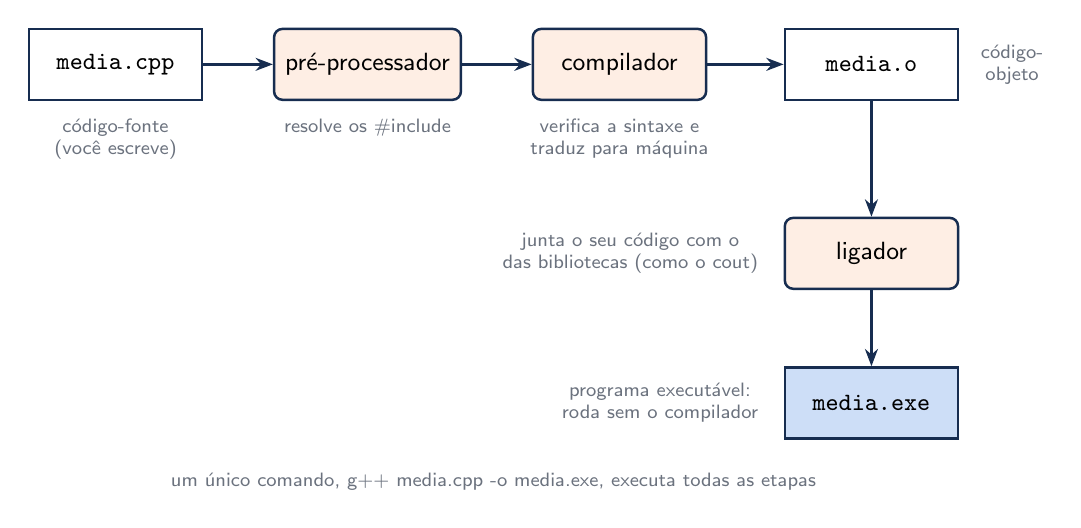
\begin{tikzpicture}
  \node[arquivo] (fonte) at (0, 0) {media.cpp};
  \node[nota, below=1mm of fonte] {código-fonte\\(você escreve)};
  \node[etapa] (pre) at (3.2, 0) {pré-processador};
  \node[nota, below=1mm of pre] {resolve os \#include};
  \node[etapa] (comp) at (6.4, 0) {compilador};
  \node[nota, below=1mm of comp] {verifica a sintaxe e\\traduz para máquina};
  \node[arquivo] (obj) at (9.6, 0) {media.o};
  \node[nota, right=1.5mm of obj] {código-\\objeto};
  \node[etapa] (lig) at (9.6, -2.4) {ligador};
  \node[nota, left=2mm of lig] {junta o seu código com o\\das bibliotecas (como o cout)};
  \node[arquivo, fill=azul] (exe) at (9.6, -4.3) {media.exe};
  \node[nota, left=2mm of exe] {programa executável:\\roda sem o compilador};
  \draw[fluxo] (fonte) -- (pre);
  \draw[fluxo] (pre) -- (comp);
  \draw[fluxo] (comp) -- (obj);
  \draw[fluxo] (obj) -- (lig);
  \draw[fluxo] (lig) -- (exe);
  \node[legenda] at (4.8, -5.3)
    {um único comando, g++ media.cpp -o media.exe, executa todas as etapas};
\end{tikzpicture}
\end{document}
